\documentclass[10pt,twocolumn,letterpaper]{article}

\usepackage{cvpr}
\usepackage{times}
\usepackage{epsfig}
\usepackage{graphicx}
\usepackage{amsmath}
\usepackage{amssymb}

% Include other packages here, before hyperref.

% If you comment hyperref and then uncomment it, you should delete
% egpaper.aux before re-running latex.  (Or just hit 'q' on the first latex
% run, let it finish, and you should be clear).
\usepackage[pagebackref=true,breaklinks=true,letterpaper=true,colorlinks,bookmarks=false]{hyperref}

%%%%%%%%% PAPER ID  - PLEASE UPDATE
\def\cvprPaperID{----} % *** Enter the CVPR Paper ID here
\def\httilde{\mbox{\tt\raisebox{-.5ex}{\symbol{126}}}}

\begin{document}

%%%%%%%%% TITLE - PLEASE UPDATE
\title{Chinese Character Style Transfer with conditional GAN}  % **** Enter the paper title here

\maketitle
\thispagestyle{empty}


%%%%%%%%% BODY TEXT - ENTER YOUR RESPONSE BELOW
\section{Introduction}

We propose a model which transforms a character from a typeface $A$ to another typeface $B$ given a few character pairs written in $A$ and $B$ respecitvely. We uses conditional GAN (cGAN) \cite{Authors01} to generate stylized character image with unaltered text meaning.

%-------------------------------------------------------------------------

\subsection{Motivation}
Unlike typefaces for English characters, it takes tremondous effort to design new Chinese typefaces. This is due to the simple fact that there are more than 4,000 commonly used Chinese characters \cite{Authors02} that have to be designed. Using this model, only a few reference style characters have to be designed manually. The model can generate the rest with consistent style. 

%------------------------------------------------------------------------
\section{Related Work}

Some of the previous methods use backpropagation on an initial random noise image \cite{Authors03} or train a feedforward network \cite{Authors04} to transfer low-level texture style from a reference image to another. There are also exceptional result on articist or photorealistic image generation and translation using GANs and its derivatives \cite{Authors05}\cite{Authors06}. 

%-------------------------------------------------------------------------
\section{Method}

\subsection{Formulation}
In this model, a generator $G$ and a discriminator $D$ will be trained. The given sample transform is $T:{A\to B}$ where $A$ and $B$ are small subset of the characters in two typefaces. $G$ will take $T$ and another character $C_A$ in typeface $A$ as input to generate an image $C_B$. $D$ then learns to discrimate between $C_B$ and other characters in typeface $B$ with $C_A$ as input. 

Note that $C_A$ acts as the constraint vector in the cGAN such that the discriminator will be able to tell the difference between a transformed version of $C_A$ and a random character that has the appearance of typeface $B$. Without this constraint, \textit{model collapse} will happen as there are a lot of freedom in the Chinese character model.

\begin{figure}[t]
	\begin{center}
		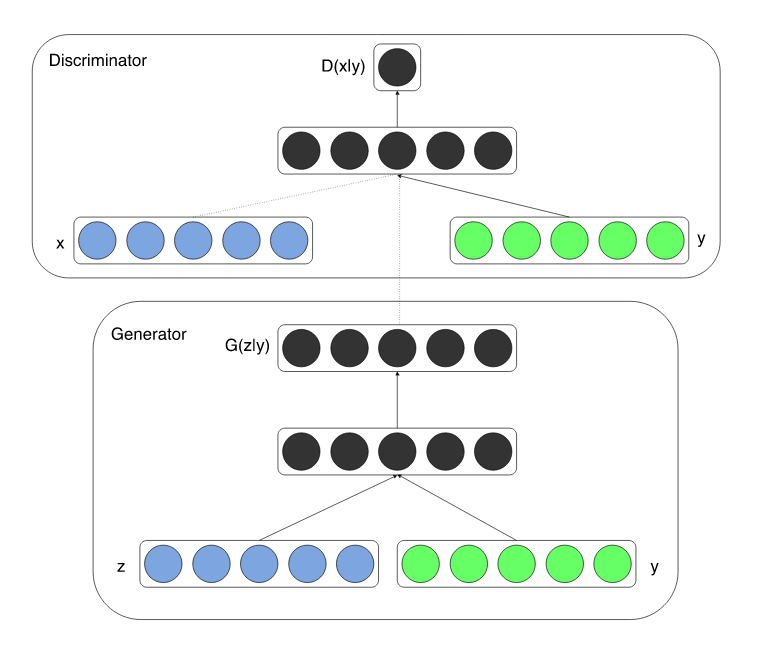
\includegraphics[width=0.8\linewidth]{img.png}
	\end{center}
	\caption{Conditional GAN. Taken from \cite{Authors01} In our model, $C_A$ acts as the $y$ vector in the figure.}
	\label{fig:long}
	\label{fig:onecol}
\end{figure}

\subsection{Data}
There are abundant free Chinese fonts available online for download in .ttf format. The images of the characters can be extracted from the font file. A few of the typefaces will be reserved for testing and validation purposes. To make the generation more stable and the fact that we will generate $C_A$ automatically from character encodings, the typeface $A$ can be fixed. In this case, we consider using MingLiU, a common typeface that has clear strokes



{\small
\bibliographystyle{ieee}
\bibliography{bib}
}

\end{document}
